\documentclass[12pt]{article}
\usepackage{amsmath, amssymb, graphicx}
\usepackage{geometry}
\usepackage{enumitem}
\usepackage{hyperref}
\geometry{a4paper, margin=1in}

\begin{document}

\title{Homework 2}
\author{Hao Yin}
\date{\today}
\maketitle

\section*{Question 1}
    \begin{enumerate}[label=\roman*.]
        \item (a)
        \[G(s) = \frac{4s-8}{s^2+2s-9}\]
        \[\text{DC GAIN} = G(0) = \frac{-8}{-9}\]

        (b)
        \[G(s) = \frac{10}{s^2+2s+10}\]
        \[\text{DC GAIN} = G(0) = \frac{10}{10} = 1\]

        \item (a)
        \[N(0) = s^2+2s-9 = 0\]
        \[\text{Poles:} s = -1 \pm \sqrt{10}\]
        \[Real(s) = -1 + \sqrt{10} > 0, \text{so this system is unstable.}\]

        (b)
        \[N(0) = s^2+2s+10 = 0\]
        \[\text{Poles:} s = -1 \pm 3i\]
        \[Real(s) = -1 < 0, \text{so this system is stable.}\]

        \item (a)
        
        From TF, we get the ODE:
        \[\ddot{y(t)} + 2\dot{y(t)} - 9y(t) = 4\dot{u(t)} - 8u(t)\]
        Guess that: $y(t) = Ce^{st}, \dot{y(t)} = Cse^{st}, 
            \ddot{y(t)} = Cs^2e^{st}$
        So we get:
        \[Cs^2e^{st} + 2Cse^{st} - 9Ce^{st} = 0\]
        \[Ce^{st} (s^2 + 2s - 9) = 0\]
        \[s = -1 \pm \sqrt{10}\]
        \[y(t) = c_1e^{(-1+\sqrt{10})t} + c_2e^{(-1-\sqrt{10})t}\]

        (b)

        From TF, we get the ODE:
        \[\ddot{y(t)} + 2\dot{y(t)} + 10y(t) = 10u(t)\]
        Guess that: $y(t) = Ce^{st}, \dot{y(t)} = Cse^{st}, 
            \ddot{y(t)} = Cs^2e^{st}$
        So we get:
        \[Cs^2e^{st} + 2Cse^{st} + 10Ce^{st} = 0\]
        \[Ce^{st} (s^2 + 2s + 10) = 0\]
        \[s = -1 \pm 3i\]
        \[y(t) = c_1e^{-t}cos(3t) + c_2e^{-t}sin(3t)\]

        \item (a)
        Roots: $s = -1 \pm \sqrt{10}$

        Homogeneous Solution: 
        \[y_h(t) = c_1e^{(-1+\sqrt{10})t} + c_2e^{(-1-\sqrt{10})t}\]

        Input: $u(t) \equiv 2$

        \[\ddot{y_p(t)} + 2\dot{y_p(t)} - 9y_p(t) = -16\]

        Guess $y_p(t) = C$ , need: $-9C = -16$ ,and then get: $C = \frac{16}{9}$

        So general form of Input response:

        \[y(t) = y_h(t) + y_p(t) = c_1e^{(-1+\sqrt{10})t} + c_2e^{(-1-\sqrt{10})t} + 
            \frac{16}{9}\]

        (b)
        Roots: $s = -1 \pm 3i$

        Homogeneous Solution: 
        \[y(t) = c_1e^{-t}cos(3t) + c_2e^{-t}sin(3t)\]

        Input: $u(t) \equiv 2$

        \[\ddot{y(t)} + 2\dot{y(t)} + 10y(t) = 20\]

        Guess $y_p(t) = C$ , need: $10C = 20$ ,and then get: $C = 2$

        So general form of Input response:

        \[y(t) = y_h(t) + y_p(t) = c_1e^{-t}cos(3t) + c_2e^{-t}sin(3t) + 2\]

        \item (a)
        For the zero initial conditions: $y(0) = 0, \dot{y(0)} = 0$

        We get:
        \[y(0) = c_1 + c_2 + \frac{16}{9} = 0\]
        \[\dot{y(0)} = (-1+\sqrt{10})c_1 + (-1-\sqrt{10}c_2) = 0\]

        So:
        \[c_1 = -1.17, c_2 = -0.6078\]

        So input response:
        \[y(t) = -1.17e^{(-1+\sqrt{10})t} -0.6078e^{(-1-\sqrt{10})t} + 
            \frac{16}{9}\]


        (b)
        For the zero initial conditions: $y(0) = 0, \dot{y(0)} = 0$

        We get:
        \[y(0) = c_1 + 2 = 0\]
        \[\dot{y(0)} = -c_1 + 3c_2 = 0\]

        So:
        \[c_1 = -2, c_2 = -2/3\]

        So input response:
        \[y(t) = -2e^{-t}cos(3t) - \frac{2}{3}e^{-t}sin(3t) + 2\]


    \end{enumerate}

\section*{Question 2}
    \begin{enumerate}[label=\alph*]
        \item TF:
        \[G(s) = \frac{4}{s+3}\]
        \[\text{Roots: } s = -3 < 0 \text{So this system is stable.}\]
        
        \item Poles: $s = -3$
        \[\text{Time constant: } \tau = \frac{1}{|Re(p)|} = \frac{1}{3}s\]

        \item y(0) = 0:
        \begin{center}
            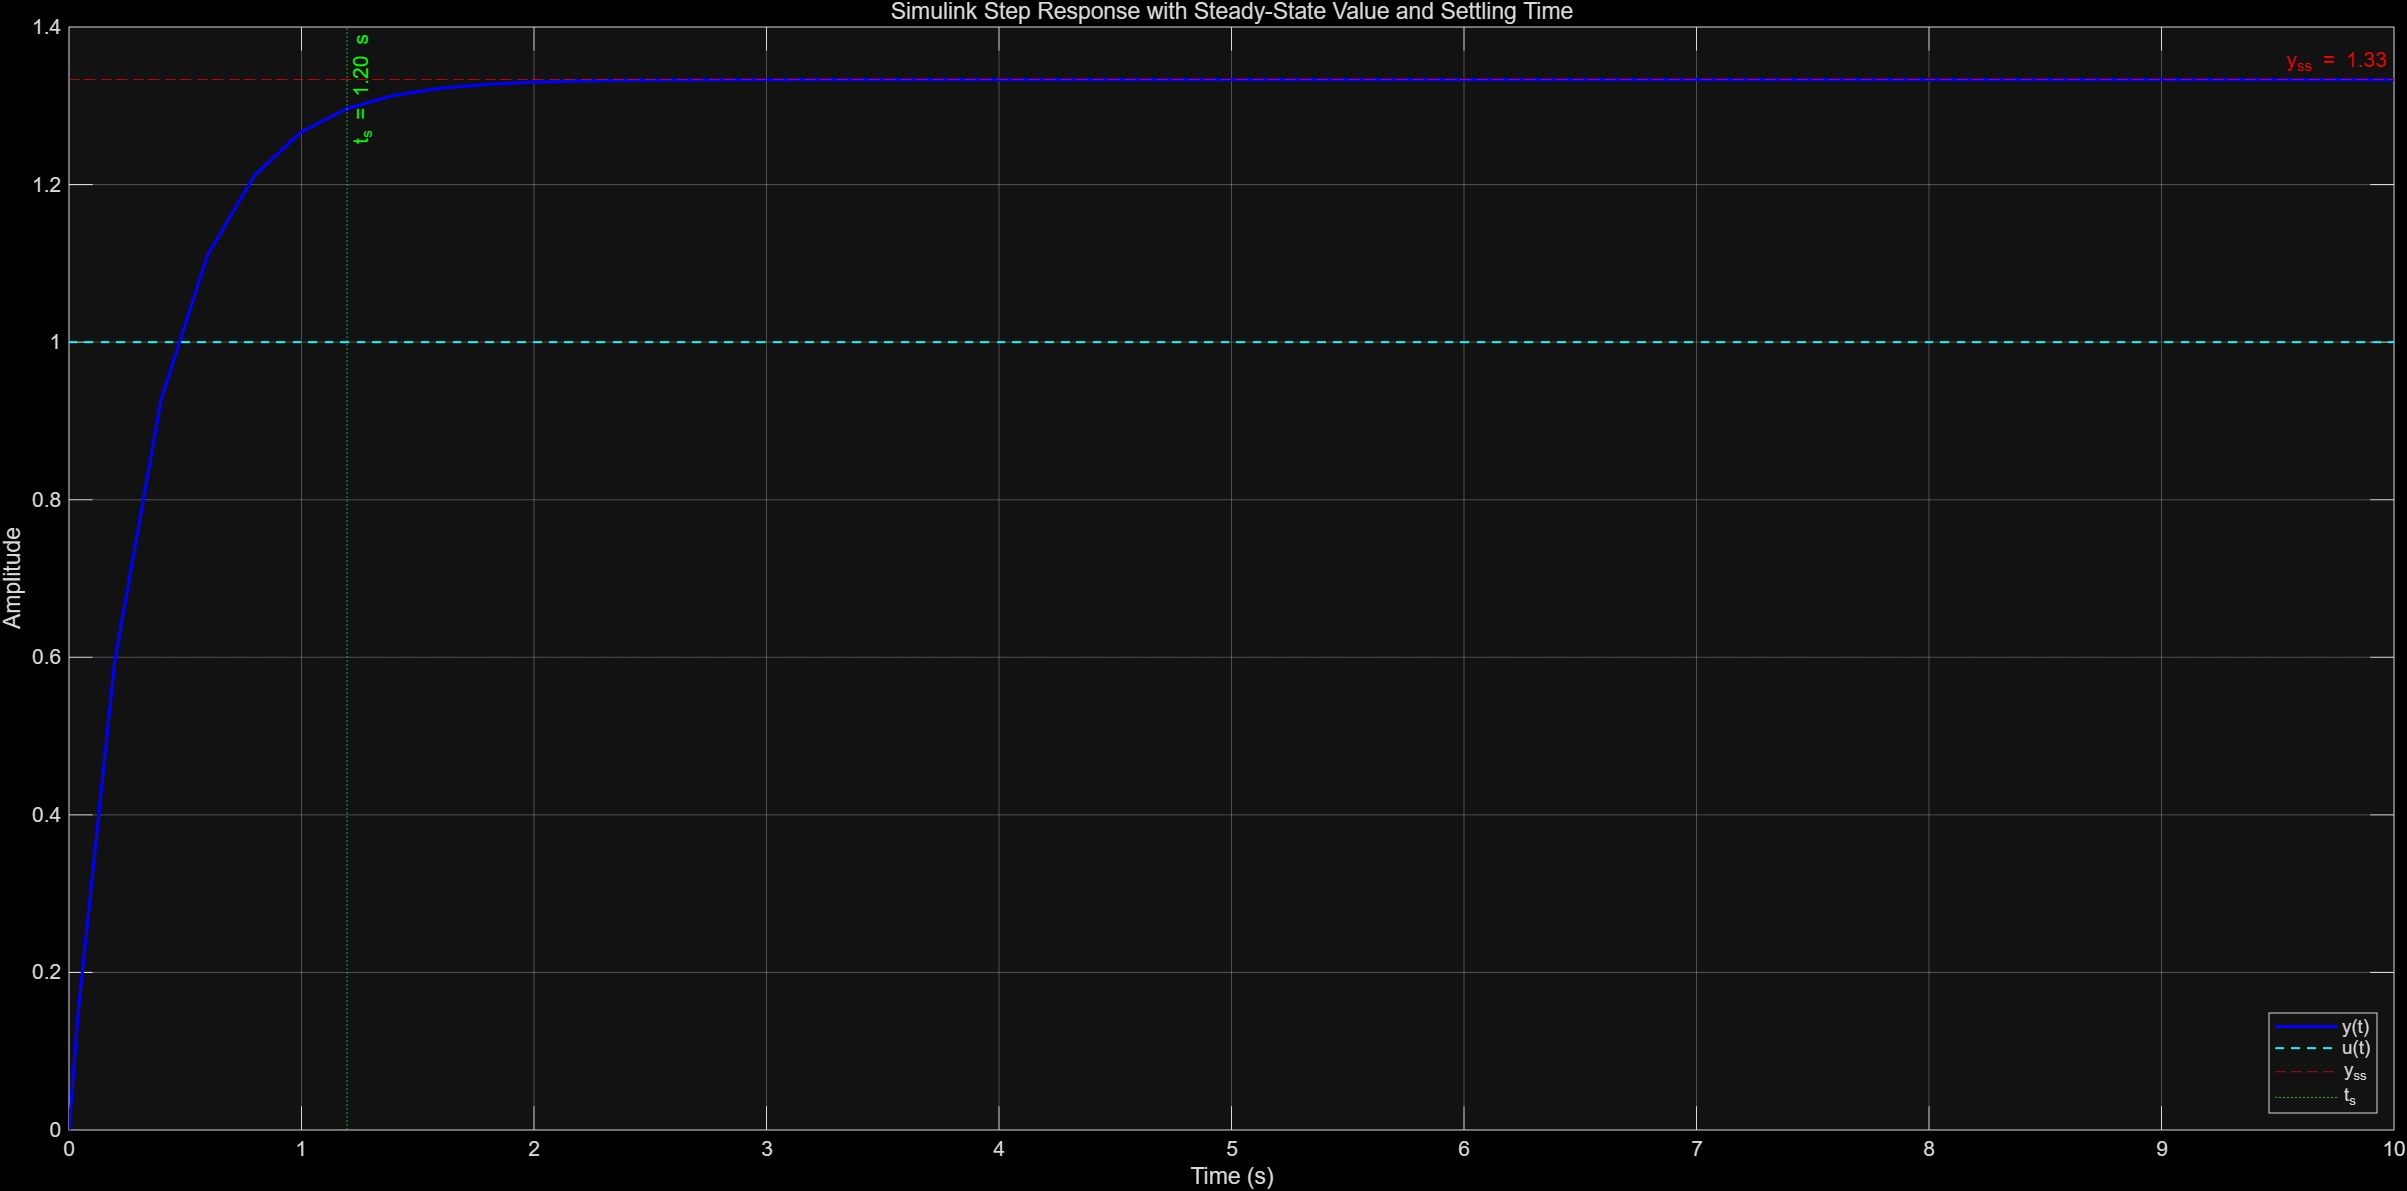
\includegraphics[width=0.6\textwidth]{Q2c.png}
        \end{center}

        \item y(0) = 1:
        \begin{center}
            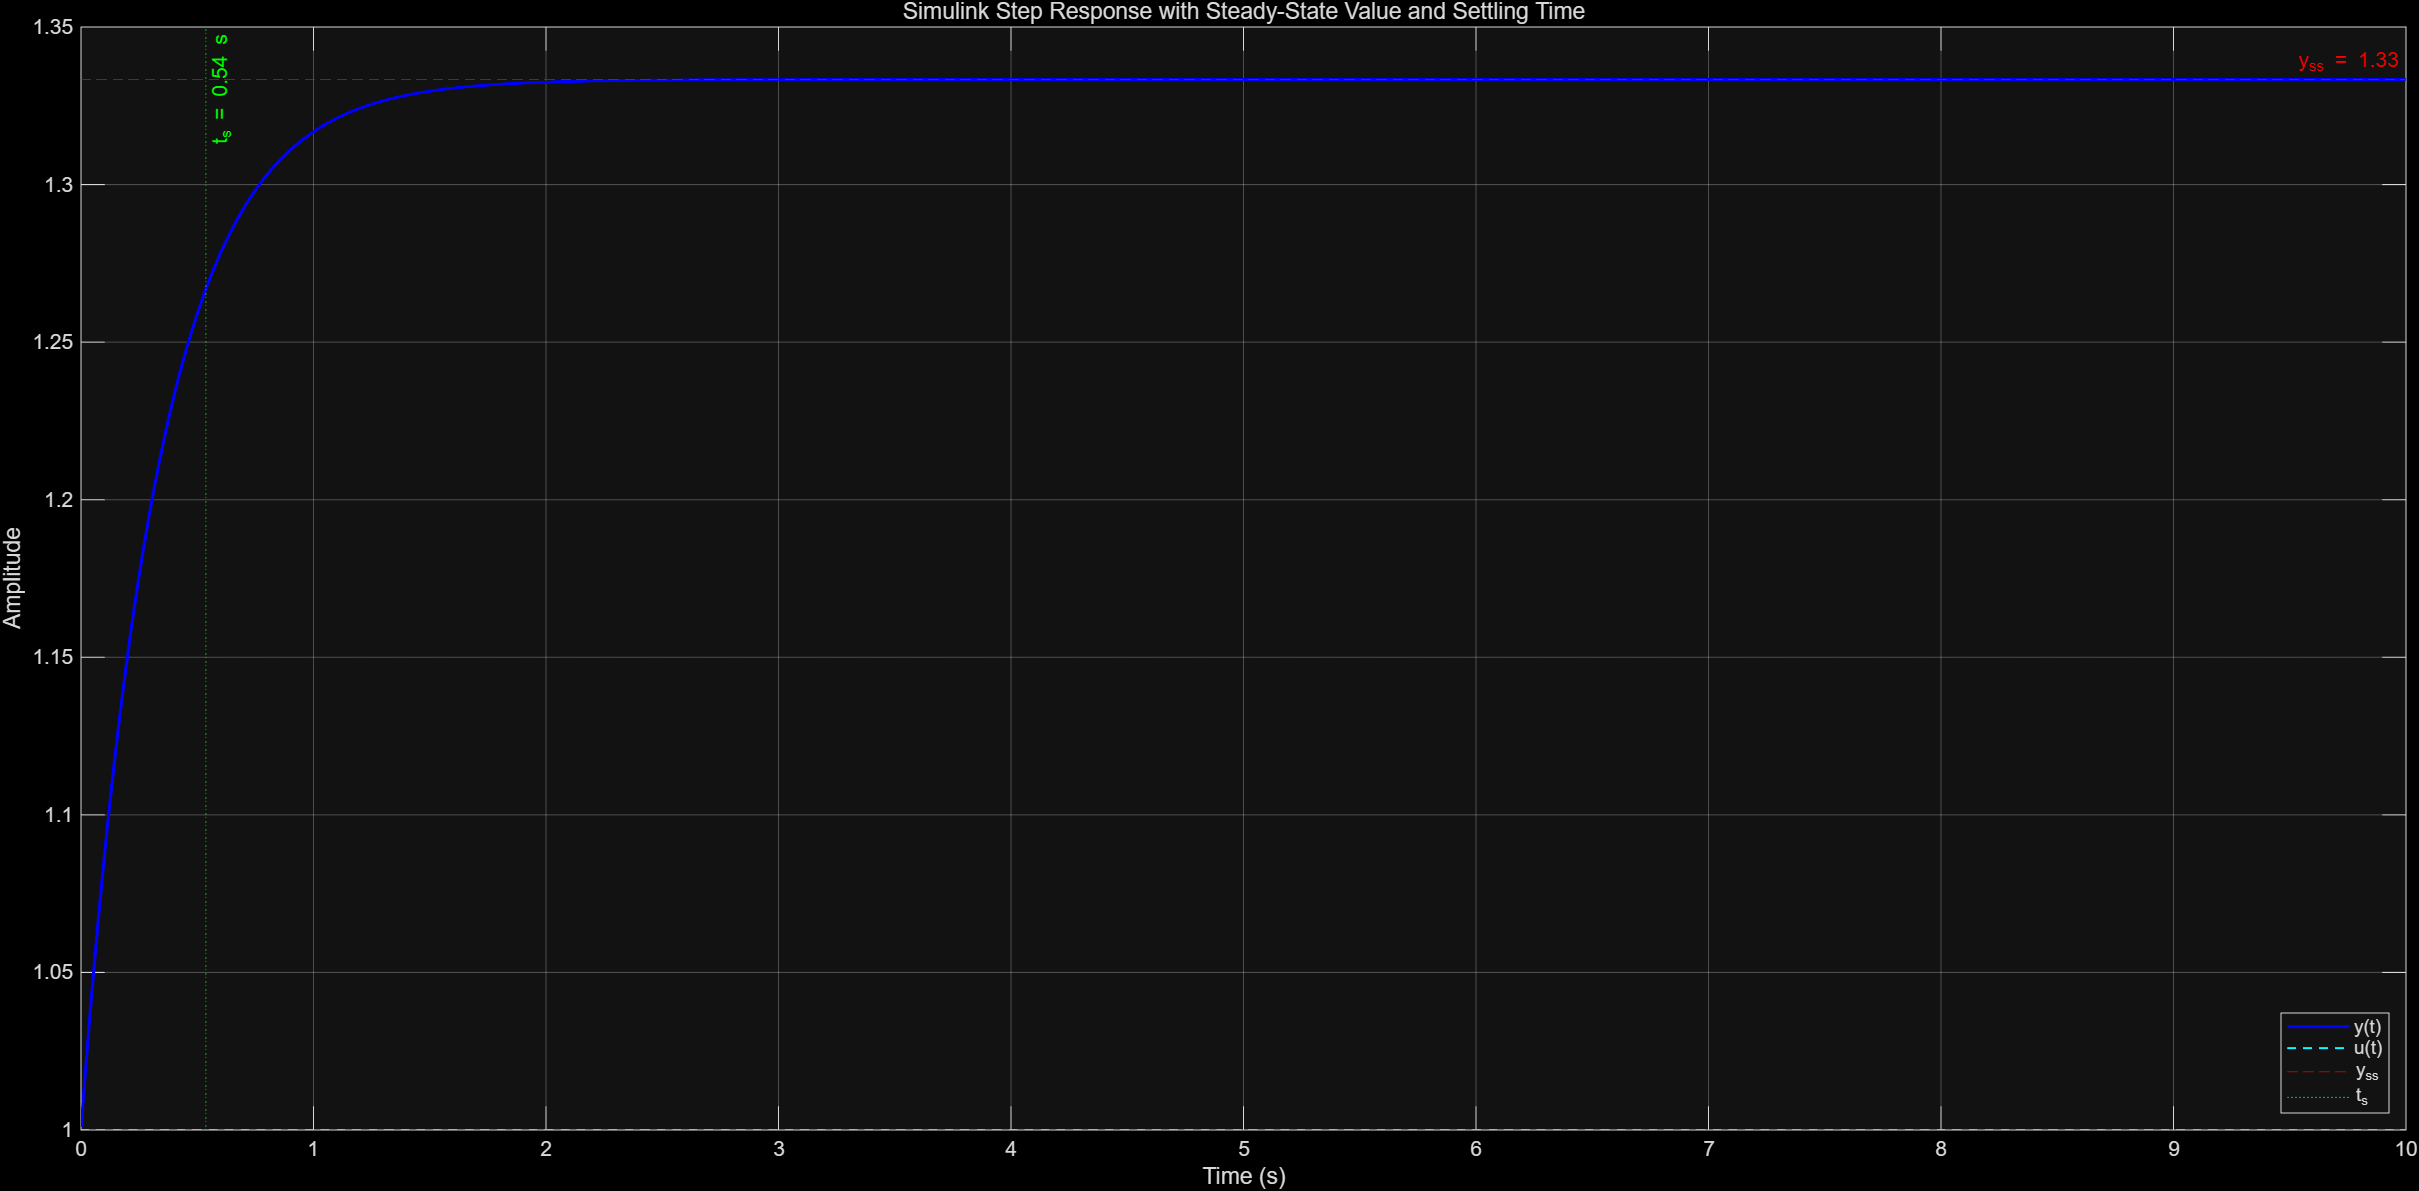
\includegraphics[width=0.6\textwidth]{Q2d.png}
        \end{center}

    \end{enumerate}

\section*{Question 3}
    \begin{enumerate}[label=\roman*.]
        \item (a) TF:
        \[G(s) = \frac{12}{s^2+2s+10}\]
        \[2\zeta\omega_n = 2, \omega_n^2 = 10\]
        \[\omega_n = \sqrt{10}, \zeta = \frac{1}{\sqrt{10}} \approx 0.3162 < 1\]
        So the system is under-damped.
        (b) TF:
        \[G(s) = \frac{8}{s^2+20s+4}\]
        \[2\zeta\omega_n = 20, \omega_n^2 = 4\]
        \[\omega_n = 2, \zeta = 5 > 1\]
        So the system is over-damped.

        \item (a)
        \[T_s \approx \frac{3}{\zeta\omega_n} = 3s\]
        (b)
        This is a over-damped system, and usually the settling time of a 
        over-damped system can be obtain from simulation which is told by 
        professor on piazza and recommended book (Control system: 
        An introduction). But I found a way to estimate the settling time of a
        over-damped system on the internet called
        \href{https://electronics.stackexchange.com/questions/511722/
        how-to-estimate-settling-time-of-an-overdamped-system}
        {Dominant pole method}, from which we can get an approximate value
        without simulation:
        \[T_s \approx \frac{3}{|Re(P_d)|} = \frac{3}{0.202} = 14.8515s\]
        Also, for verification, result from simulation:
        \[T_s = 14.8792\]

        \item (a)
        \[M = e^{\frac{-\zeta}{\sqrt{1-\zeta^2}}\pi} = 0.3509 = 35.09\%\]
        (b)
        For it is over-damped system, there is nop overshoot and $M = 0$

        \item (a) From iii, $M = 35.09, \text{step value} = 2, \text{DC Gain}
        =1.2, y_{ss} = 2.4$
        So $\text{Peak Value} = 2.4 * (1+0.3509) = 3.2422$
        And from picture, $\text{Peak Value} = 3.242$ which is corresponding to
        the result we get from iii.
        \begin{center}
            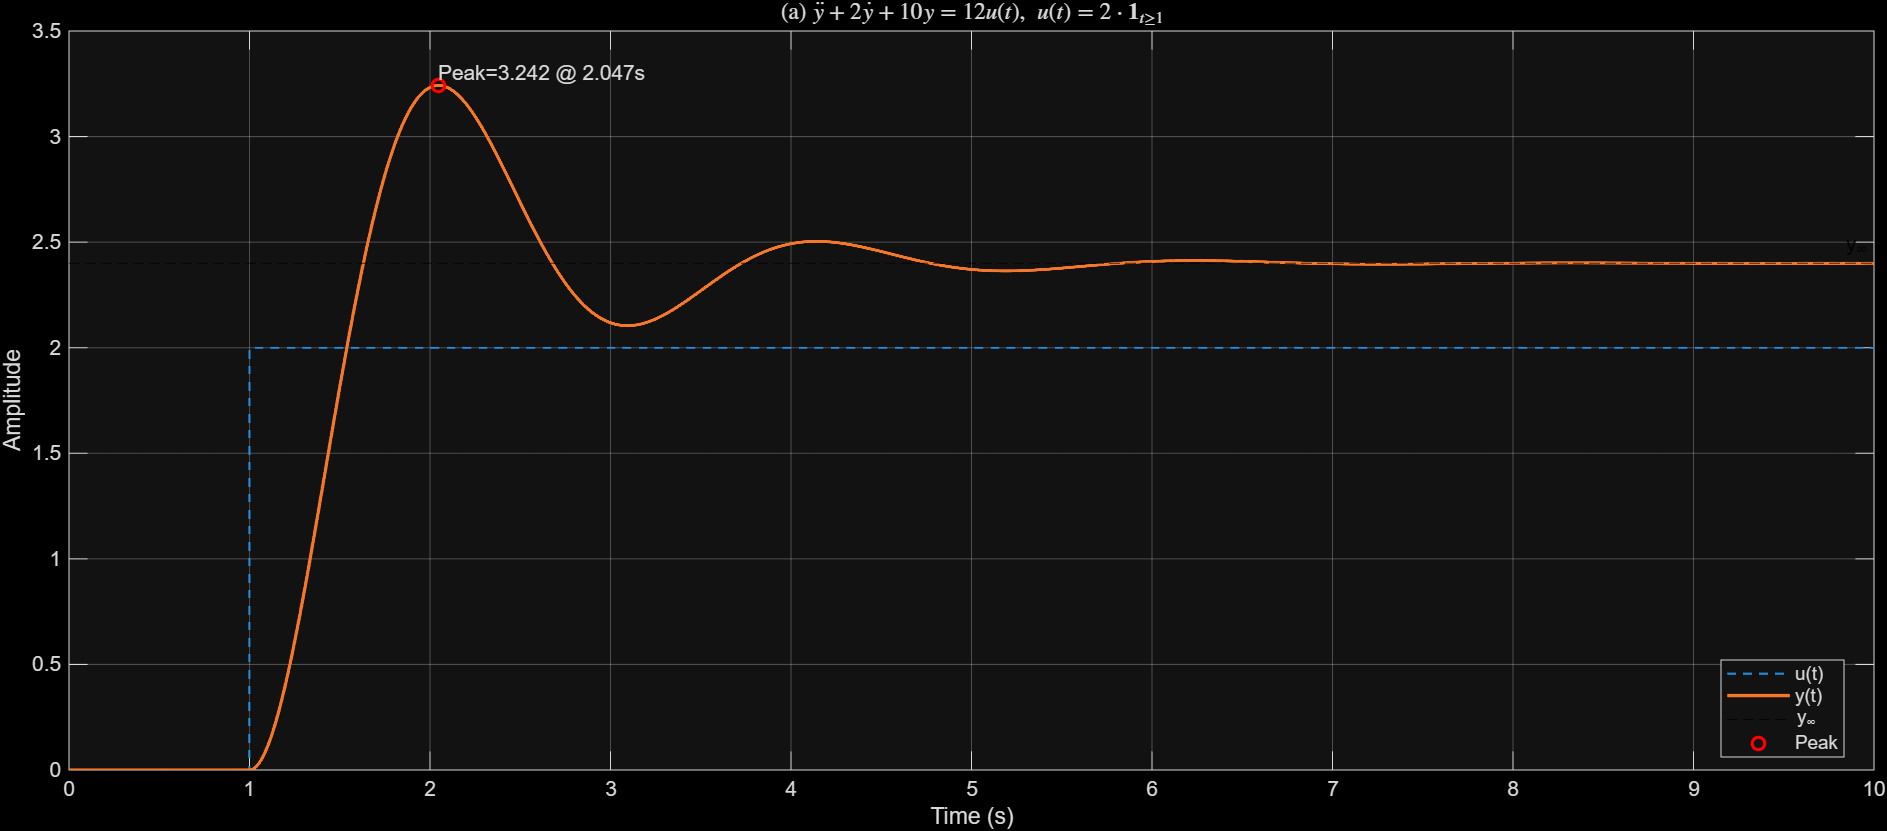
\includegraphics[width=0.6\textwidth]{Q3a.png}
        \end{center}

        (b) From iii, $M = 0, \text{step value} = 2, \text{DC Gain}
        =2, y_{ss} = 4$
        So $\text{Peak Value} = 4 * (1+0) = 4$
        And from picture, $\text{Peak Value} = 4$ which is also corresponding to
        the result we get from iii.
        \begin{center}
            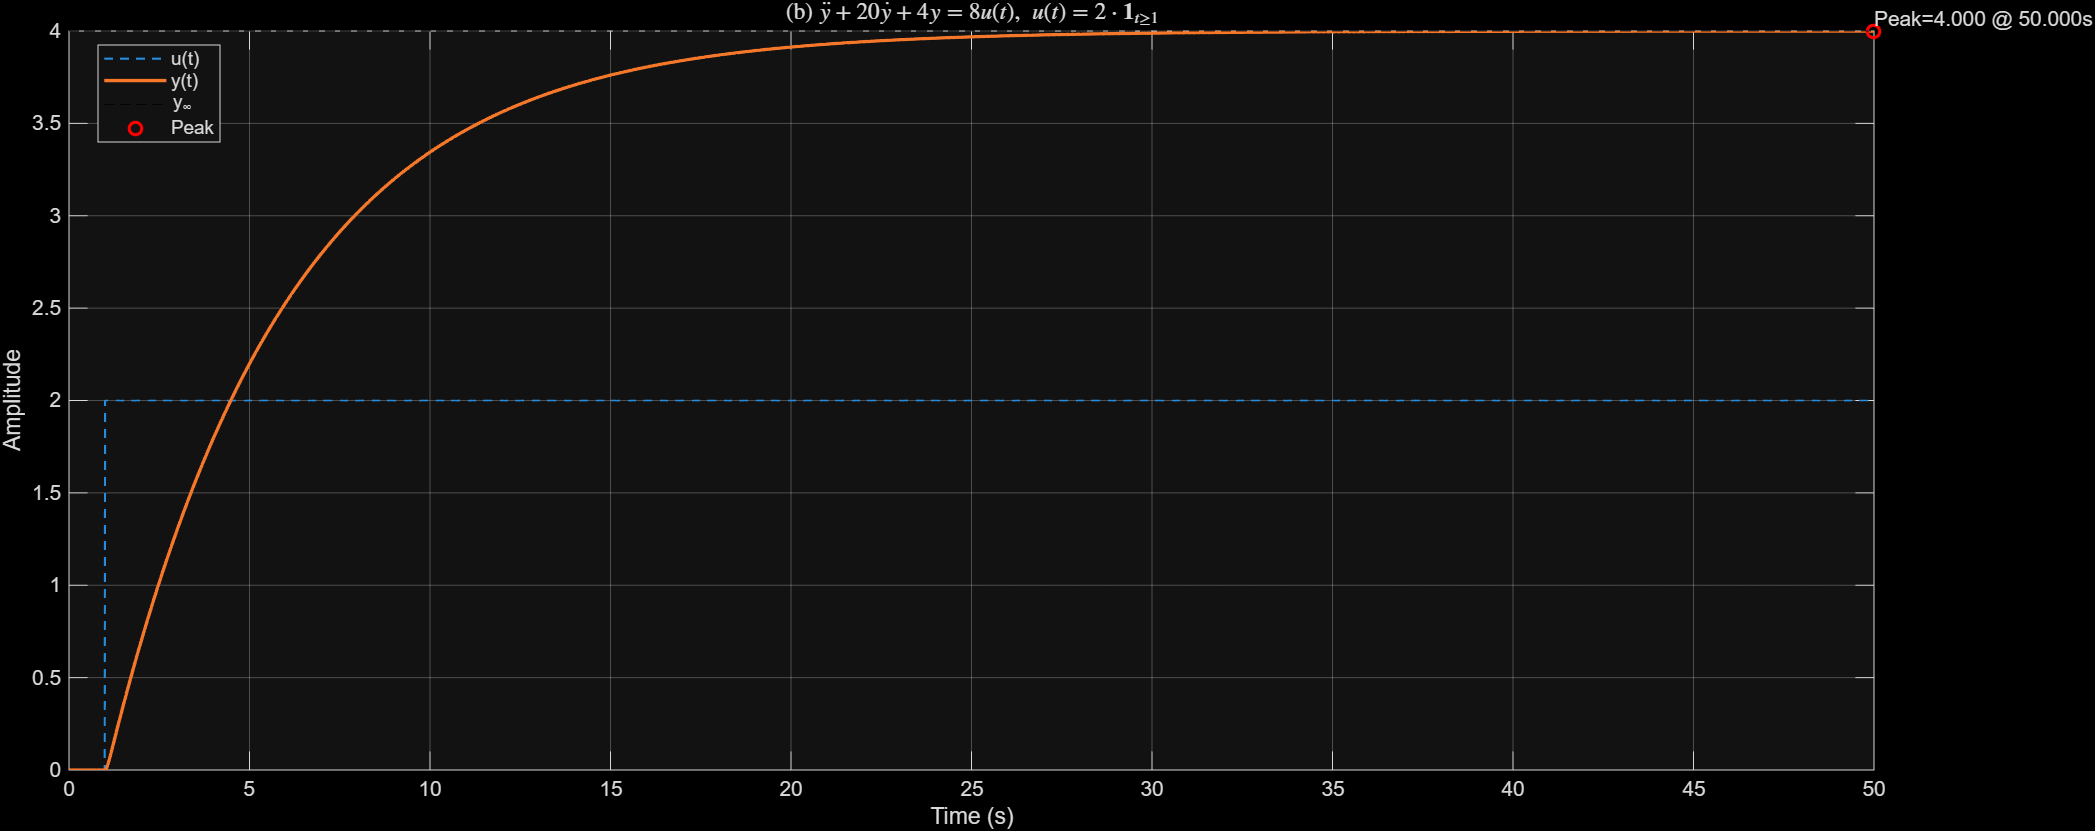
\includegraphics[width=0.6\textwidth]{Q3b.png}
        \end{center}

    \end{enumerate}

\section*{Question 4}
    \begin{enumerate}[label=\alph*]
        \item \[G(s) = \frac{8000}{s^5 + 77s^4 +2051s^3 + 21325s^2 + 80000s +
            406250}\]
        \[\text{Poles:} s_1 = s_2 = s_3 = -25, s_4 = -1+5i, s_5 = -1-5i\]

        \item \[\tau_1 = \tau_2 = \tau_3 = 0.04, \tau_4 = \tau_5 = 1\]
        
        \item A second-order approximation because the poles i choose is 
            complex.

        \item \[G_a(s) = \frac{b_0}{s^2+2s+26}\]
        \[G_a(0) = \frac{b_0}{26} = \frac{8000}{406250}\]
        \[b_0 = 0.512\]
        \[G_a(0) = \frac{0.512}{s^2+2s+26}\]

        \item The step response:
        \begin{center}
            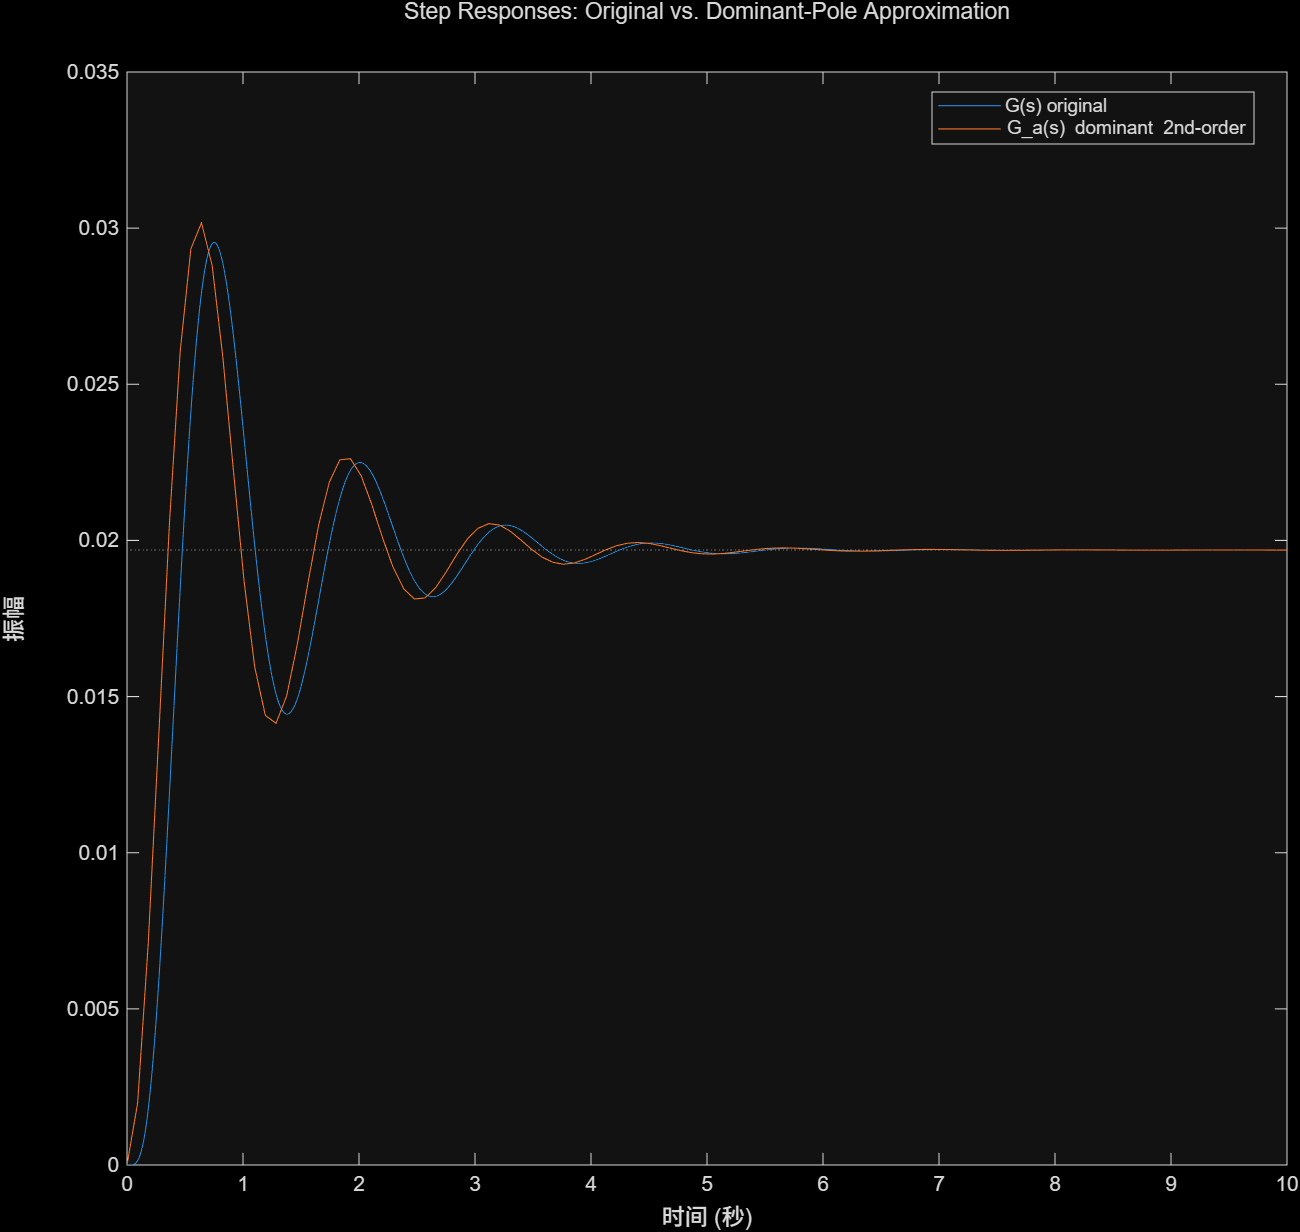
\includegraphics[width=0.6\textwidth]{Q4.png}
        \end{center}

    \end{enumerate}

\section*{Question 5}
    \begin{enumerate}[label=\alph*]
        \item \[H(s) = \frac{8000}{s^5 + 637s^4 + 7571s^3 + 44685s^2 + 194400s +
            406250}\]
        \[\text{Poles:} s_1 = -625, s_2 = 1+5i, s_3 = 1-5i, s_4 = s_5 = -5\]

        \item \[\tau_1 = 0.0016, \tau_2 = \tau_3 = 1, \tau_4 = \tau_5 = 0.2\]

        \item \[H_a(s) = \frac{b_0}{s^2+2s+26}\]
        \[H_a(0) = \frac{b_0}{26} = \frac{8000}{406250}\]
        \[b_0 = 0.512\]
        \[H_a(0) = \frac{0.512}{s^2+2s+26}\]

    \end{enumerate}

\section*{Question 6}
    When they have the same poles 1, $G_a(s)$ is better because the other poles 
        are 0.04, which is smaller enough than $H_a(s)$ which is 0.2.

\section*{Question 7}

    \[DC GAIN = J(0) = \frac{a_0}{10}\]
    Consider the step value is 1 as conventional: $\frac{a_0}{10}  = 5$
    \[a_0 = 50\]
    Then from simulation on MATLAB, tuning the value of $a_1$, get $a_1 = -51$
    \begin{center}
        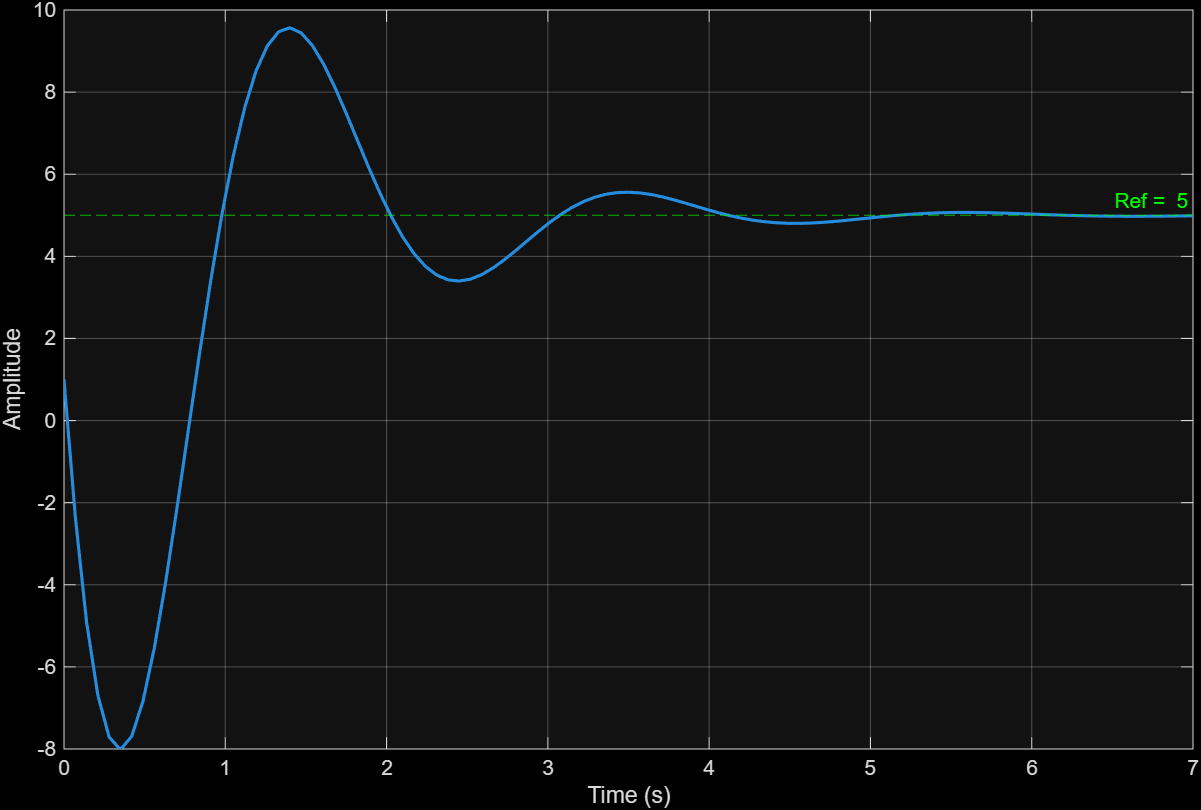
\includegraphics[width=0.6\textwidth]{Q7.png}
        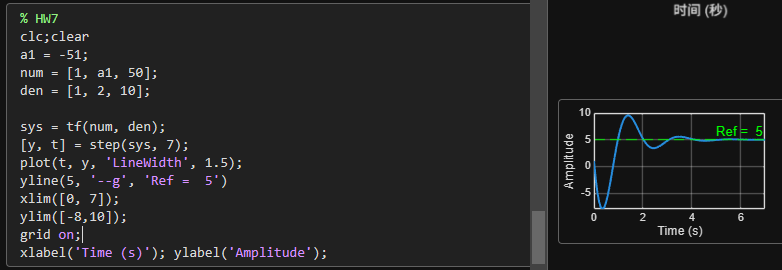
\includegraphics[width=0.6\textwidth]{Q7m.png}
    \end{center}

\end{document}